\autsection{Submarine}{Paul Connetable}

The penetrator will be anchored at the bottom of the ice crust, on the top of Europa's ocean, in order to find life. Still, if there is indeed life on Europa, there is a very high probability to find it and evidence of it at the bottom of the ocean. Any dead form of life would eventually sink at the bottom of this ocean, creating there a layer of sediments, mud and and thus, nutrients. The friction of water on the rocky core could also increase the water temperature near the bottom, creating there another very likely place for life development. This is why being able to send a probe, even small, to the bottom of Europa's ocean would add a crucial tool for finding life, or clues indicating the presence of life.


From another point of view, any further information found about Europa, even if it is not life related. It is for example of uttermost importance to understand better the physics and the system functioning to obtain measurements of the water flow, temperature, salinity at different depths, and to get water samples distant from the penetrator position.


To execute these missions, the best suited tool is a little submarine. This little submarine would be stored inside the penetrator, and released when the penetrator  reaches the ocean. These submarines would be made in titanium, and could contain any combination of instruments wanted. They would be some measurement platforms designed for smaller diverse missions, thanks to their versatility. They would communicate the results or the data to the penetrator either by direct liaison with it thanks to an optical fiber, or by sonar, or by bluetooth (for smaller ranges). In the case of sonar use, the penetrator could receive the signal thanks to the antenna placed at its bottom, which is used during the descent.

\autsubsection{Spherical submarines}{Paul Connetable}

In this part are presented the results obtained for the weight and the wall thickness of small spherical submarines, in function of their outer radius. In order to find these results, we used the titanium alloy presented in the Material subsection. We used here a factor of safety of 2, meaning that the maximum stress obtained at the maximum depth is half of the alloy yield stress, here 410 MPa. In this simulation, we size the submarines so that they can go to a 50 km depth, which represents an external pressure of 80 MPa. In order to be accurate, we did not use the thin-walled assumtion for spherical vessels, but the full formulas, defined by the following stresses:

\begin{equation}
\sigma_{tt}=\frac{P_{a}\times R_{a}^{3}-P_{b}\times R_{b}^{3}}{R_{b}^{3}-R_{a}^{3}}-\frac{(P_{a}-P_{b}) \times R_{b}^{3} R_{a}^{3}}{(R_{b}^{3}-R_{a}^{3}) \times R^{3}}
\end{equation}

\begin{equation}
\sigma_{\theta\theta}=\frac{P_{a}\times R_{a}^{3}-P_{b}\times R_{b}^{3}}{R_{b}^{3}-R_{a}^{3}}+\frac{(P_{a}-P_{b}) \times R_{b}^{3} R_{a}^{3}}{2 \times (R_{b}^{3}-R_{a}^{3}) \times R^{3}}
\end{equation}

Moreover, in this specific case, while applying the symmetries of the problem, the equivalent stress obtained with the Von Mises criterion is:

\begin{equation}
\sigma_{equivalent}= abs(\sigma_{tt}-\sigma_{\theta\theta})
\end{equation}

In these equations, $R_{a}$, $R_{b}$, $P_{a}$, $P_{b}$, and R are respectively: The inner radius, the outer radius, the internal pressure, the external pressure and the radius where the stress is computed. The results obtained are presented in figures \ref{wallthickness} and \ref{sphereweight}. the matlab code used to produce these figures is presented in Annex \ref{spherecode}.


\begin{figure}[H]
\centering
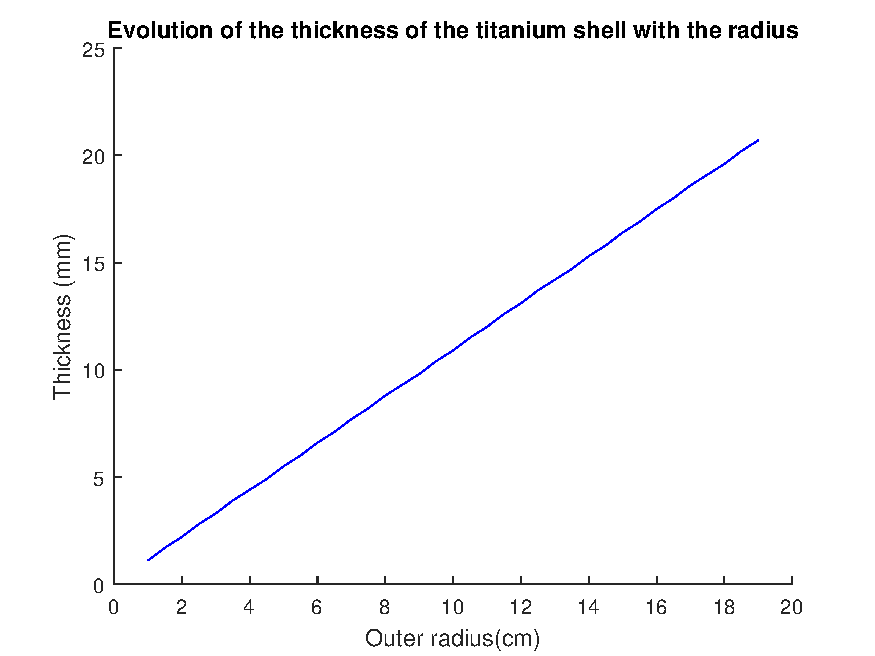
\includegraphics[width=10cm, height=10cm, clip]{figures/Paul/Thickness.pdf}
\caption{Thickness of the titanium wall in function of the outer radius of the submarine}
\label{wallthickness}
\end{figure}

\begin{figure}[H]
\centering
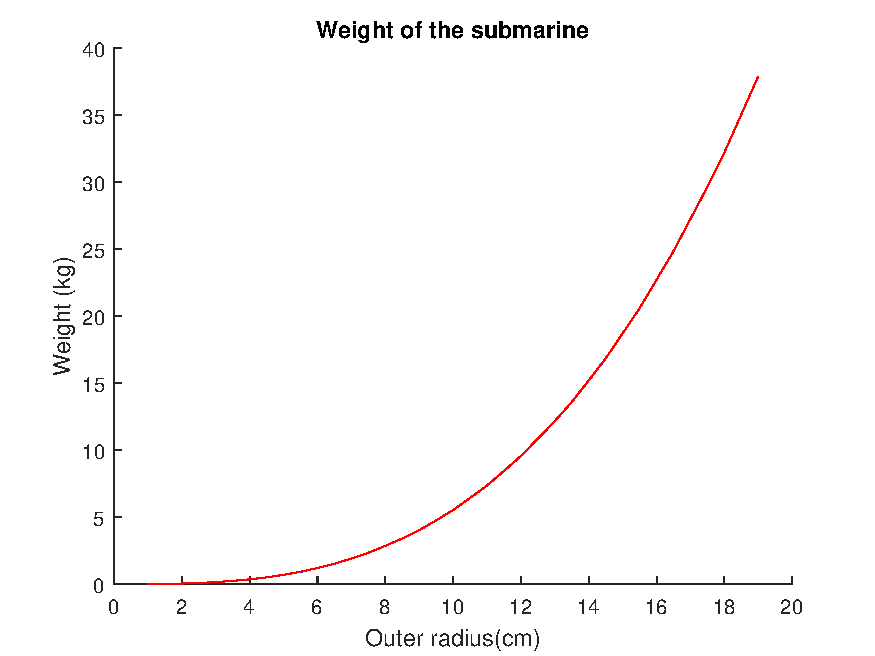
\includegraphics[width=10cm, height=10cm, clip]{figures/Paul/SphereWeight.pdf}
\caption{Weight of the spherical submarine in function of its outer radius}
\label{sphereweight}
\end{figure}

It appears that the walls of the spherical submarine were thin enough so that the results match with the thin wall assumption, since the thickness has a linear relation with the outer radius.
One can observe that small submarines would be very light, and can go at significant depth. Since most of the instruments can be put out of the sphere, the inner part of it would mainly be used for electronics such as computers and batteries and thus wouldn't need to be too big. It is possible to significantly reduce the weight of such a submarine by increasing its internal pressure. If the inner parts of the submarine can handle higher pressure, it is very interesting to increase this pressure. However, this part of the problem has not been researched in depth, which is why we assume that the internal pressure in the spheres were of 1 bar.

The conclusion is that spherical submarines can prove themselves very useful for our life finding mission and Europa's system functioning, while being relatively light and small for basic measurements. It would therefore be very interesting to use these tools in our mission.
